
\section{Network architecture}

\begin{figure}[h]
\centering
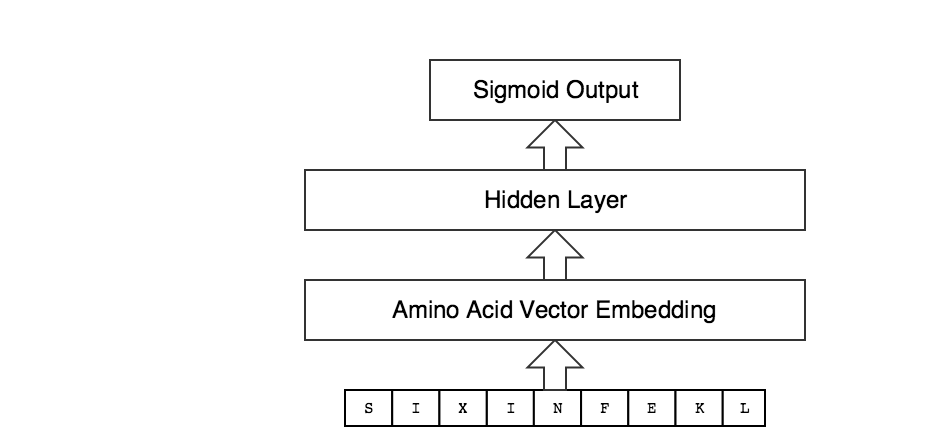
\includegraphics[scale=0.5]{figures/mhcflurry-gliffy-network.png}
\caption{Neural network architecture for predicting peptide-MHC affinities from fixed length amino acid sequences}
\end{figure}

\subsection{Predicting affinities for multiple peptide lengths using a 9mer encoding}
Reduction from multiple peptide lengths to a 9mer encoding was done using a scheme similar to that of NetMHC\cite{lundegaard2008accurate}. Peptides with only 8 amino acids were extended with the insertion of a special wildcard ``X'' at every position in the sequence. Peptides longer than 9 amino acids were shortened by removing consecutive stretches of residues at every position. These lengthened or shortened samples were included in the training set with a sample weight inversely proportional to the number of samples created from a single measurement. For prediction, non-9mer peptides are converted into 9mers using the same scheme and the prediction is the geometric mean of the 9mer predictions.